\chapter{Instructions} % Main appendix title
\label{appendixA}

Required packages: keras, sklearn, pandas, numpy, PIL, pyyaml.

split\_stack.py: The initial PAT and US images that we received were in a 3-dimensional image stack (.tif) format. This script is to quickly process these stacks and generate a corresponding set of 2D images.
The original dataset has the following directory structure:
\dirtree{%
.1 dataset.
.2 AF014.
.3 PAT 930.
.4 014 PAT 930 initial stack.tif .
.3 US.
.4 14.tif .
.2 AF018.
.2 ..
.2 ..
}
Output directory structure produced by the script:
\dirtree{%
.1 PAT\_extracted.
.2 AF014.
.3 014\_15.jpg .
.3 014\_16.jpg .
.3 014\_17.jpg .
.3 014\_18.jpg .
.3 014\_19.jpg .
.3 014\_20.jpg .
.2 AF018.
.2 ..
.2 ..
}

data.py partitions the data into k-fold, prepares the directory as needed by flow\_from\_directory() for training (this step will be done automatically in training). Directory structure is:
\dirtree{%
.1 data .
.2 train.
.3 B .
.4 014\_15.jpg .
.4 014\_16.jpg .
.4 ..
.3 C .
.4 027\_14.jpg .
.4 027\_15.jpg .
.4 ..
.2 valid.
.3 B .
.3 C .
}

trin.py: Main function, includes reading training set, k-fold partitioning, training model, and reporting training and validation loss and accuracy. A configuration YAML file should be provided to train.py. Path to dataset, model used, and many training parameters are specified in the file.


\chapter{Other Dataset}
\label{appendixB}
Due to the poor performance in experiments with our dataset, to verify that the neural network models are correctly implemented, the models are trained on other classification datasets \citep{Janowczyk2016} and \citep{catdog}.

\begin{figure}[h]
\centering
\begin{subfigure}[b]{.2\linewidth}
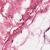
\includegraphics[width=\linewidth]{Figs/8864_idx5_x1251_y1651_class0.png}
\end{subfigure}
\begin{subfigure}[b]{.2\linewidth}
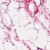
\includegraphics[width=\linewidth]{Figs/8864_idx5_x1201_y1801_class0.png}
\end{subfigure}
\begin{subfigure}[b]{.2\linewidth}
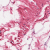
\includegraphics[width=\linewidth]{Figs/8864_idx5_x1201_y1701_class0.png}
\end{subfigure}
\begin{subfigure}[b]{.2\linewidth}
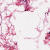
\includegraphics[width=\linewidth]{Figs/8864_idx5_x1151_y1701_class0.png}
\end{subfigure}

\begin{subfigure}[b]{.2\linewidth}
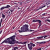
\includegraphics[width=\linewidth]{Figs/8864_idx5_x1851_y2251_class1.png}
\end{subfigure}
\begin{subfigure}[b]{.2\linewidth}
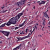
\includegraphics[width=\linewidth]{Figs/8864_idx5_x1801_y2701_class1.png}
\end{subfigure}
\begin{subfigure}[b]{.2\linewidth}
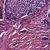
\includegraphics[width=\linewidth]{Figs/8864_idx5_x1801_y2651_class1.png}
\end{subfigure}
\begin{subfigure}[b]{.2\linewidth}
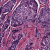
\includegraphics[width=\linewidth]{Figs/8864_idx5_x1801_y2551_class1.png}
\end{subfigure}
\caption{IDC Breast Cancer Dataset: class0 \& class1}
\label{IDC}
\end{figure}


\begin{figure}[h]
\centering
\begin{subfigure}[b]{.24\linewidth}
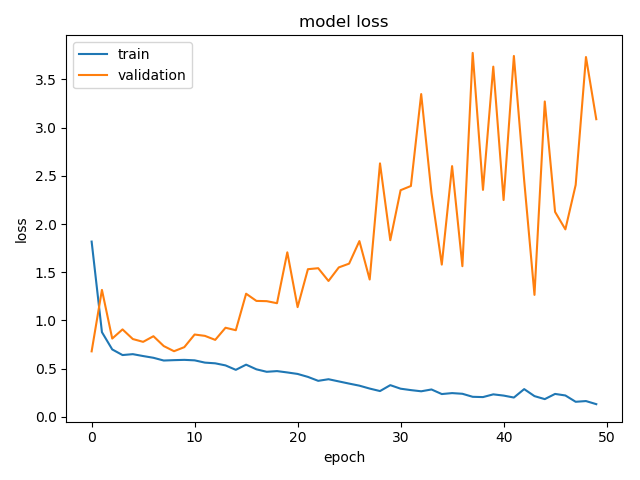
\includegraphics[width=\linewidth]{Figs/small_us_loss.jpg}
\caption{Small loss US}
\end{subfigure}
\begin{subfigure}[b]{.24\linewidth}
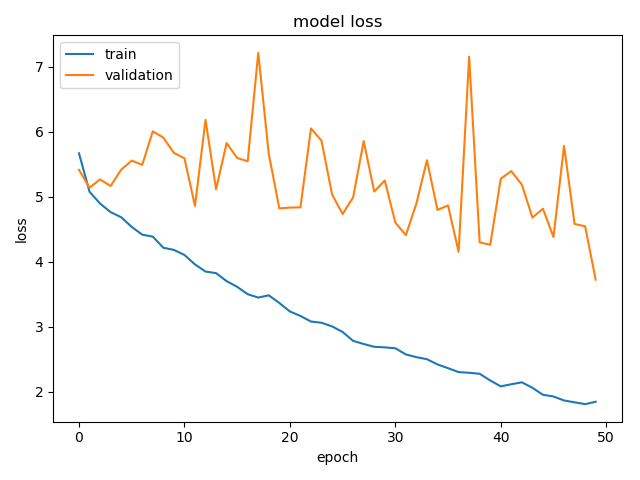
\includegraphics[width=\linewidth]{Figs/resnet_us_loss.jpg}
\caption{ResNet loss US}
\end{subfigure}
\begin{subfigure}[b]{.24\linewidth}
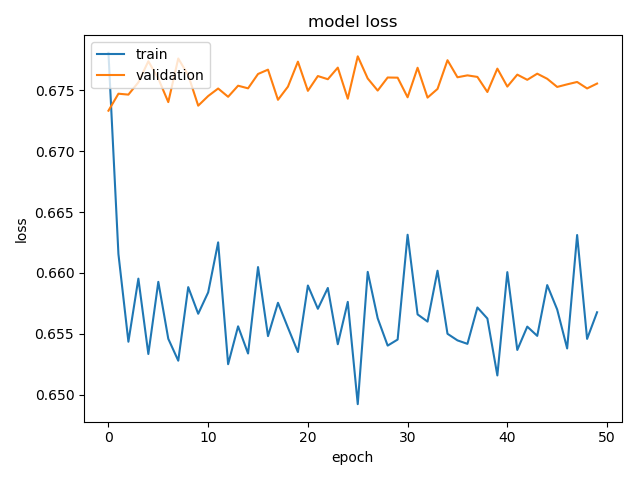
\includegraphics[width=\linewidth]{Figs/vgg_us_loss.jpg}
\caption{VGG loss US}
\end{subfigure}
\begin{subfigure}[b]{.24\linewidth}
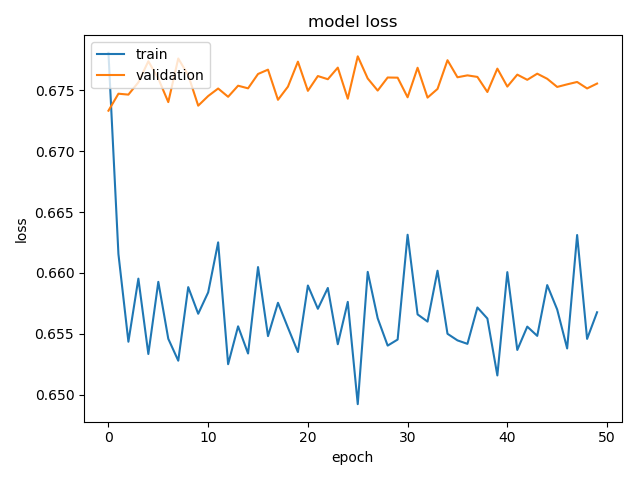
\includegraphics[width=\linewidth]{Figs/vgg_us_loss.jpg}
\caption{VGG-IN loss US}
\end{subfigure}

\begin{subfigure}[b]{.24\linewidth}
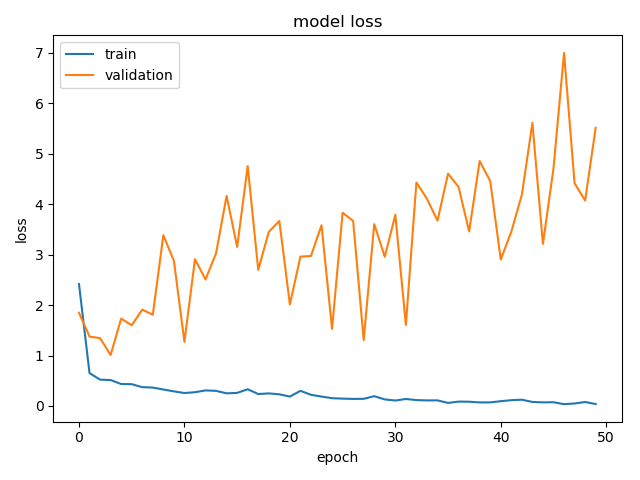
\includegraphics[width=\linewidth]{Figs/small_pat_loss.jpg}
\caption{Small loss PAT}
\end{subfigure}
\begin{subfigure}[b]{.24\linewidth}
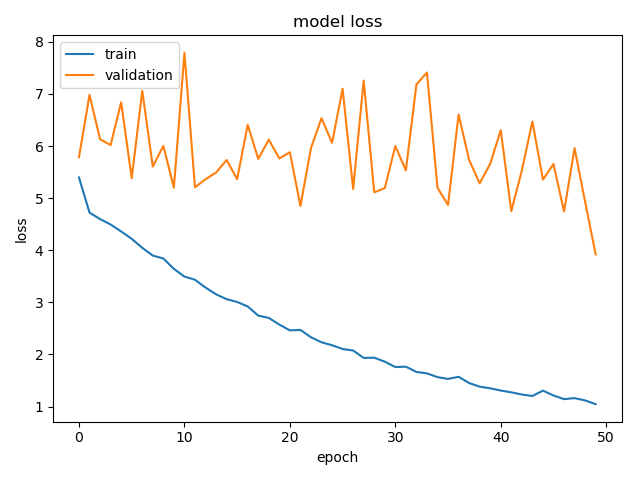
\includegraphics[width=\linewidth]{Figs/resnet_pat_loss.jpg}
\caption{ResNet loss PAT}
\end{subfigure}
\begin{subfigure}[b]{.24\linewidth}
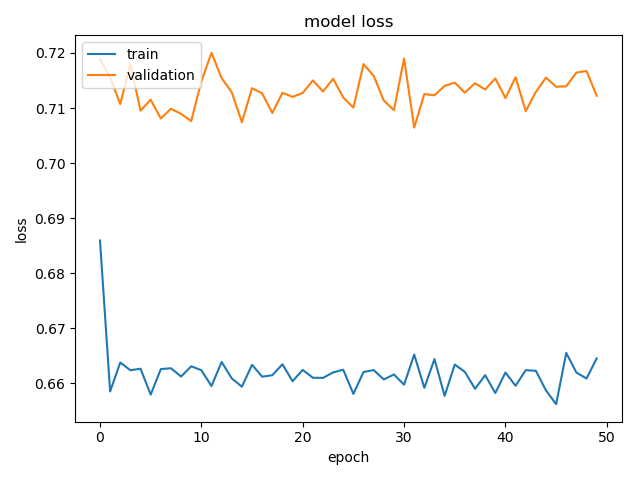
\includegraphics[width=\linewidth]{Figs/vgg_pat_loss.jpg}
\caption{VGG loss PAT}
\end{subfigure}
\begin{subfigure}[b]{.24\linewidth}
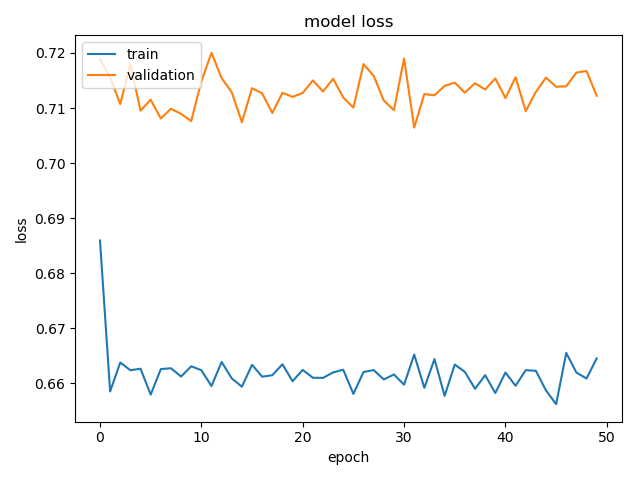
\includegraphics[width=\linewidth]{Figs/vgg_pat_loss.jpg}
\caption{VGG-IN loss PAT}
\end{subfigure}
\caption{Model loss}
\label{fig:loss2}
\end{figure}

\begin{figure}[h]
\centering
\begin{subfigure}[b]{.24\linewidth}
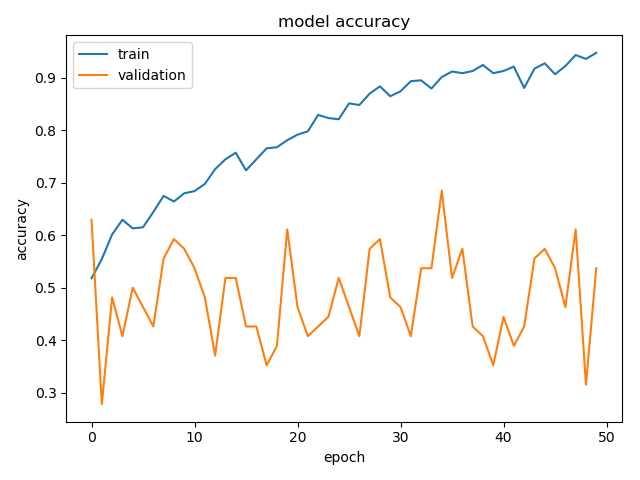
\includegraphics[width=\linewidth]{Figs/small_us_acc.jpg}
\caption{Small accuracy US}
\end{subfigure}
\begin{subfigure}[b]{.24\linewidth}
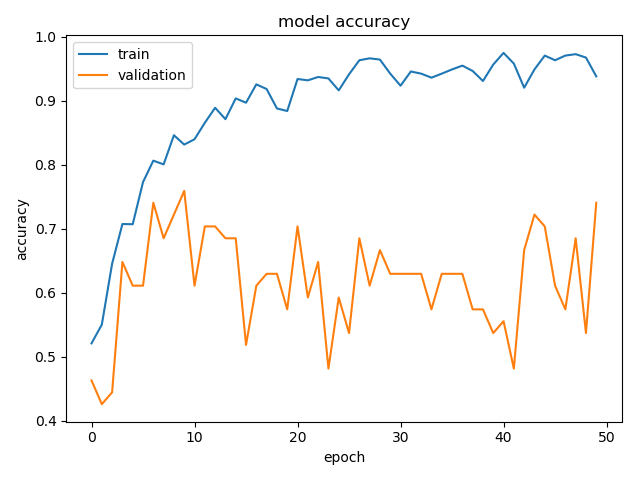
\includegraphics[width=\linewidth]{Figs/resnet_us_acc.jpg}
\caption{ResNet accuracy US}
\end{subfigure}
\begin{subfigure}[b]{.24\linewidth}
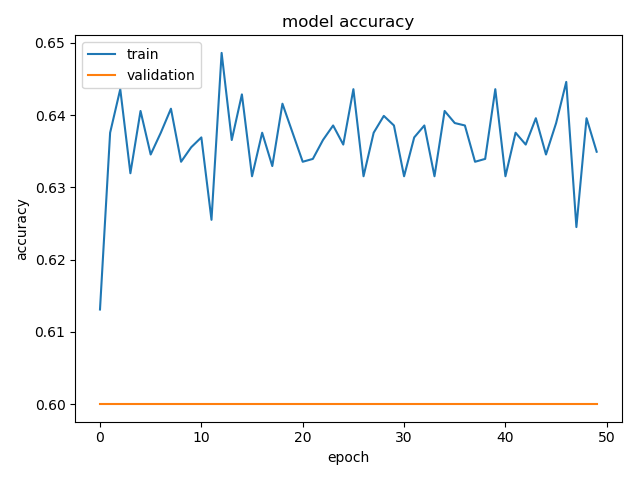
\includegraphics[width=\linewidth]{Figs/vgg_us_acc.jpg}
\caption{VGG accuracy US}
\end{subfigure}
\begin{subfigure}[b]{.24\linewidth}
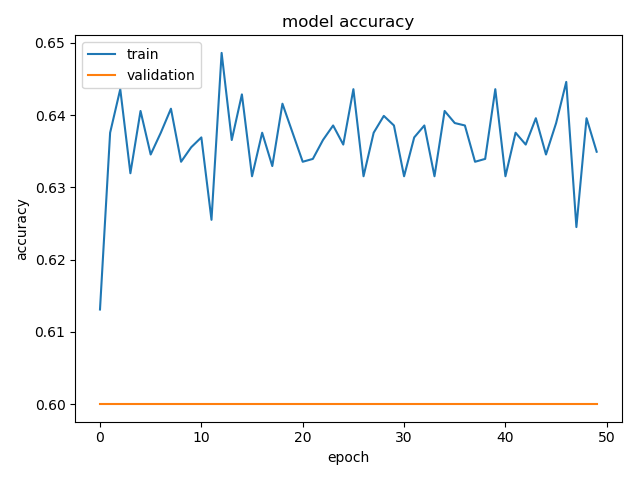
\includegraphics[width=\linewidth]{Figs/vgg_us_acc.jpg}
\caption{VGG-IN accuracy US}
\end{subfigure}

\begin{subfigure}[b]{.24\linewidth}
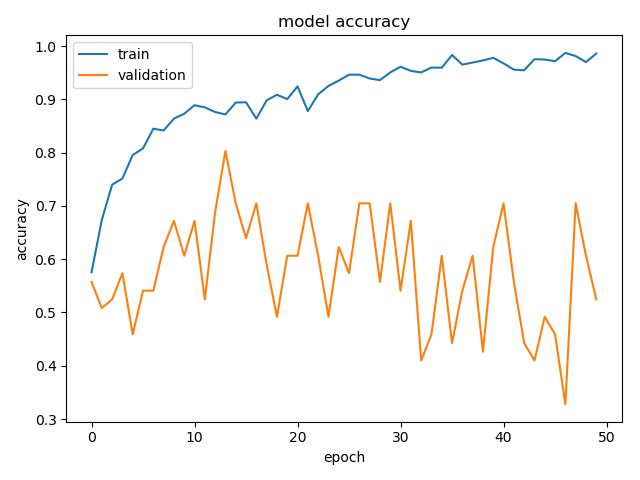
\includegraphics[width=\linewidth]{Figs/small_pat_acc.jpg}
\caption{Small accuracy PAT}
\end{subfigure}
\begin{subfigure}[b]{.24\linewidth}
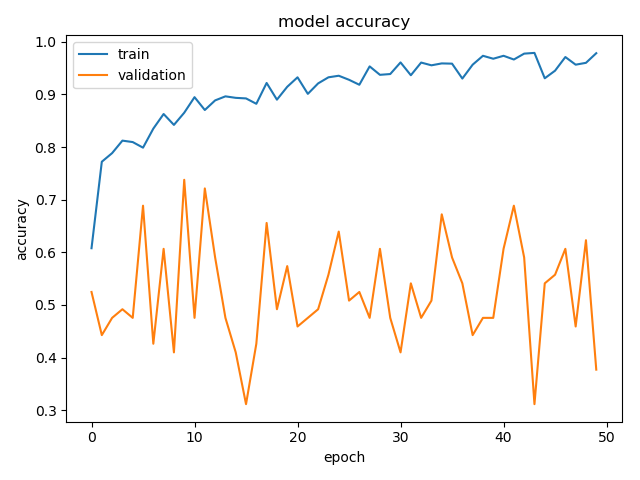
\includegraphics[width=\linewidth]{Figs/resnet_pat_acc.jpg}
\caption{ResNet accuracy PAT}
\end{subfigure}
\begin{subfigure}[b]{.24\linewidth}
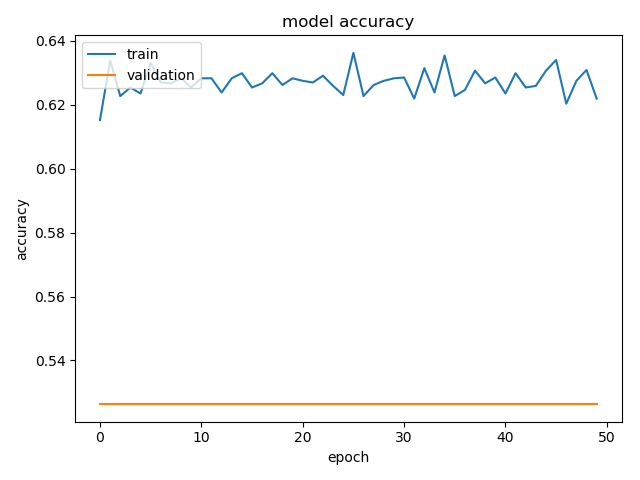
\includegraphics[width=\linewidth]{Figs/vgg_pat_acc.jpg}
\caption{VGG accuracy PAT}
\end{subfigure}
\begin{subfigure}[b]{.24\linewidth}
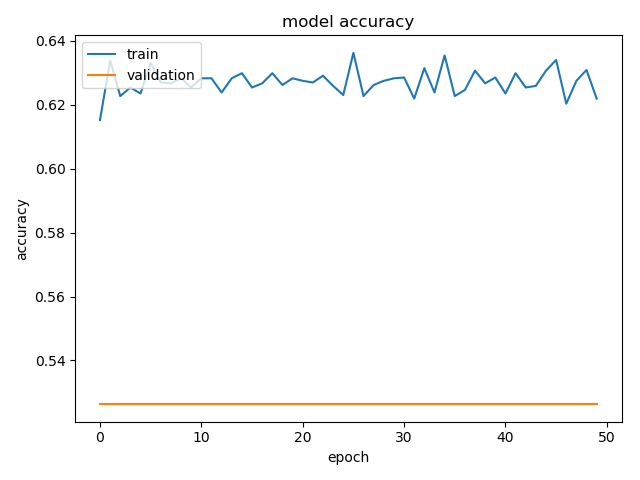
\includegraphics[width=\linewidth]{Figs/vgg_pat_acc.jpg}
\caption{VGG-IN accuracy PAT}
\end{subfigure}
\caption{Model accracy}
\label{fig:acc2}
\end{figure}

From the results, we can see that neural network models benefit from large amounts of data. The loss is decreasing and accuracy is increasing for both IDC Breast Cancer dataset and cat\&dog dataset. Accuracy and $F_1$ score is reported in Table \ref{acctable2}.


\begin{table}[h]
\centering
\begin{tabular}{ |p{3cm}||p{3cm}|p{3cm}|p{3cm}|  }
 \hline
 Model       & Accuracy & Class 0 $F_1$ score & Class 1 $F_1$ score\\
 \hline
 \hline
 Small Breast   & 0.90  & 0.94 &  0.78\\
 ResNet Breast  & 0.91  & 0.94 &  0.80\\
 VGG Breast      & 0.77  & 0.87 &  0\\
 VGG-IN breast & 0 & 0 & 0 \\
 \hline
 Small CatDog   & 0.90  & 0.94 &  0.78\\
 ResNet CatDog  & 0.91  & 0.94 &  0.80\\
 VGG CatDog      & 0.77  & 0.87 &  0\\
 VGG-IN CatDog & 0 & 0 & 0 \\
  \hline
\end{tabular}
\caption{Model accuracy and $F_1$ score}
\label{acctable2}
\end{table}
